\chapter{Model 2 Residual Diagnostics and Robustness Plots}
\label{app:diagnostics_robustness}

This appendix presents additional graphical diagnostic evaluations for Model~2 and the comparative earnings-channel robustness forest across the seven specifications R1, R2, and R4 through R8 (Specification R3 is omitted because ROA is measured on a different scale).

Figure~\ref{fig:app_robustness_forest} presents the coefficient forest plot contrasting parameter estimates and 95\% HC3 confidence intervals across these seven specifications.

\begin{figure}[!htbp]
\centering
\caption[Comparative Coefficient Forest Plot]{Comparative Coefficient Forest Plot Across Seven Robustness Specifications (R1, R2, R4--R8)}
\label{fig:app_robustness_forest}
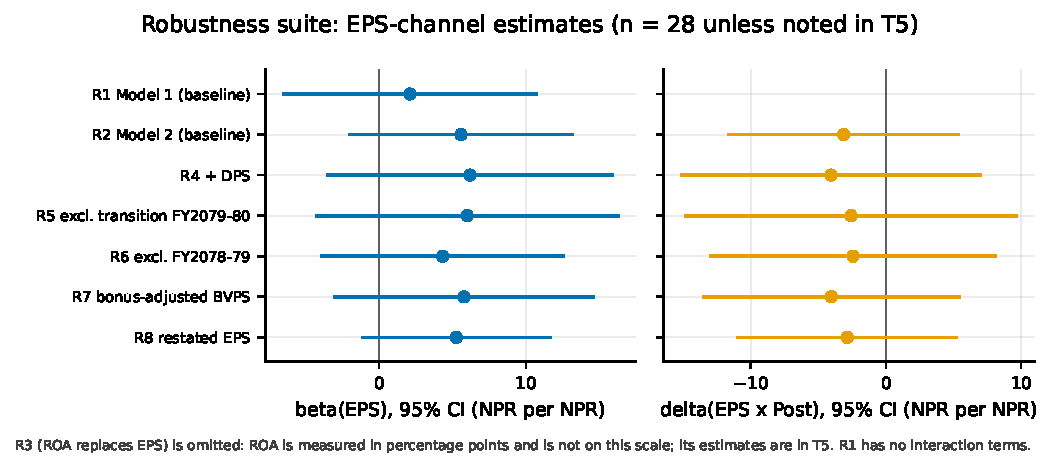
\includegraphics[width=0.88\textwidth]{figures/A2_robustness_forest.pdf}
\end{figure}

Figure~\ref{fig:app_model2_diagnostics} illustrates the four-panel econometric diagnostic suite evaluated on Model~2 residuals, examining linearity, residual normality, heteroskedasticity, and influential observations.

\begin{figure}[!htbp]
\centering
\caption{Econometric Diagnostic Panel for Model 2 Residuals}
\label{fig:app_model2_diagnostics}
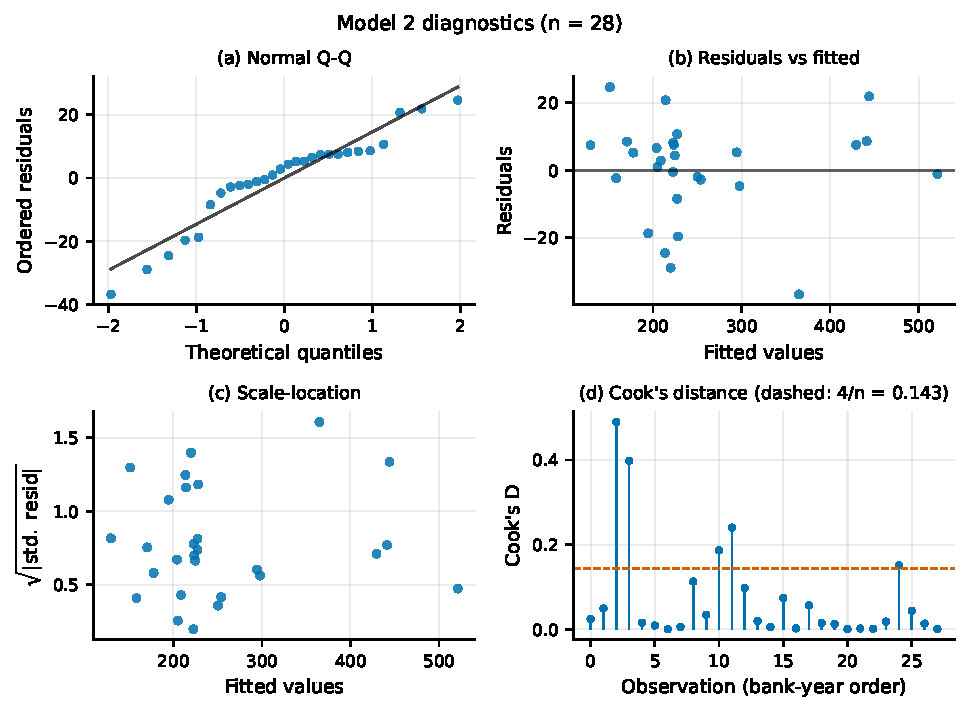
\includegraphics[width=0.88\textwidth]{figures/A3_model2_diagnostics.pdf}
\end{figure}

